\subsection{Other page client-side \& admin-side}
Let's see some screenshots of some pages of the e-commerce project that were designed with the same technique just saw.
\newline
Following shows the page order of admin-side:
\begin{figure}[htb]
\centering
\includegraphics[width=1.0\linewidth]{images/chapter4/page-order-all.png}\hfill
\caption[page order admin-side]{Page order admin-side}
\label{fig:page_order_admin_side}
\end{figure}
\newline
Following shows the page vendor of admin-side:
\begin{figure}[htb]
\centering
\includegraphics[width=1.0\linewidth]{images/chapter4/page-vendor-all.png}\hfill
\caption[page vendor admin-side]{Page vendor admin-side}
\label{fig:page_vendor_admin_side}
\end{figure}
Following shows the page coupon of admin-side:
\begin{figure}[htb]
\centering
\includegraphics[width=1.0\linewidth]{images/chapter4/page-coupon-all.png}\hfill
\caption[page vendor admin-side]{Page coupon admin-side}
\label{fig:page_coupon_admin_side}
\end{figure}
Following shows the page products of admin-side:
\begin{figure}[htb]
\centering
\includegraphics[width=1.0\linewidth]{images/chapter4/page-products-all.png}\hfill
\caption[page products admin-side]{Page products admin-side}
\label{fig:page_products_admin_side}
\end{figure}
Following shows the page products of client-side:
\begin{figure}[htb]
\centering
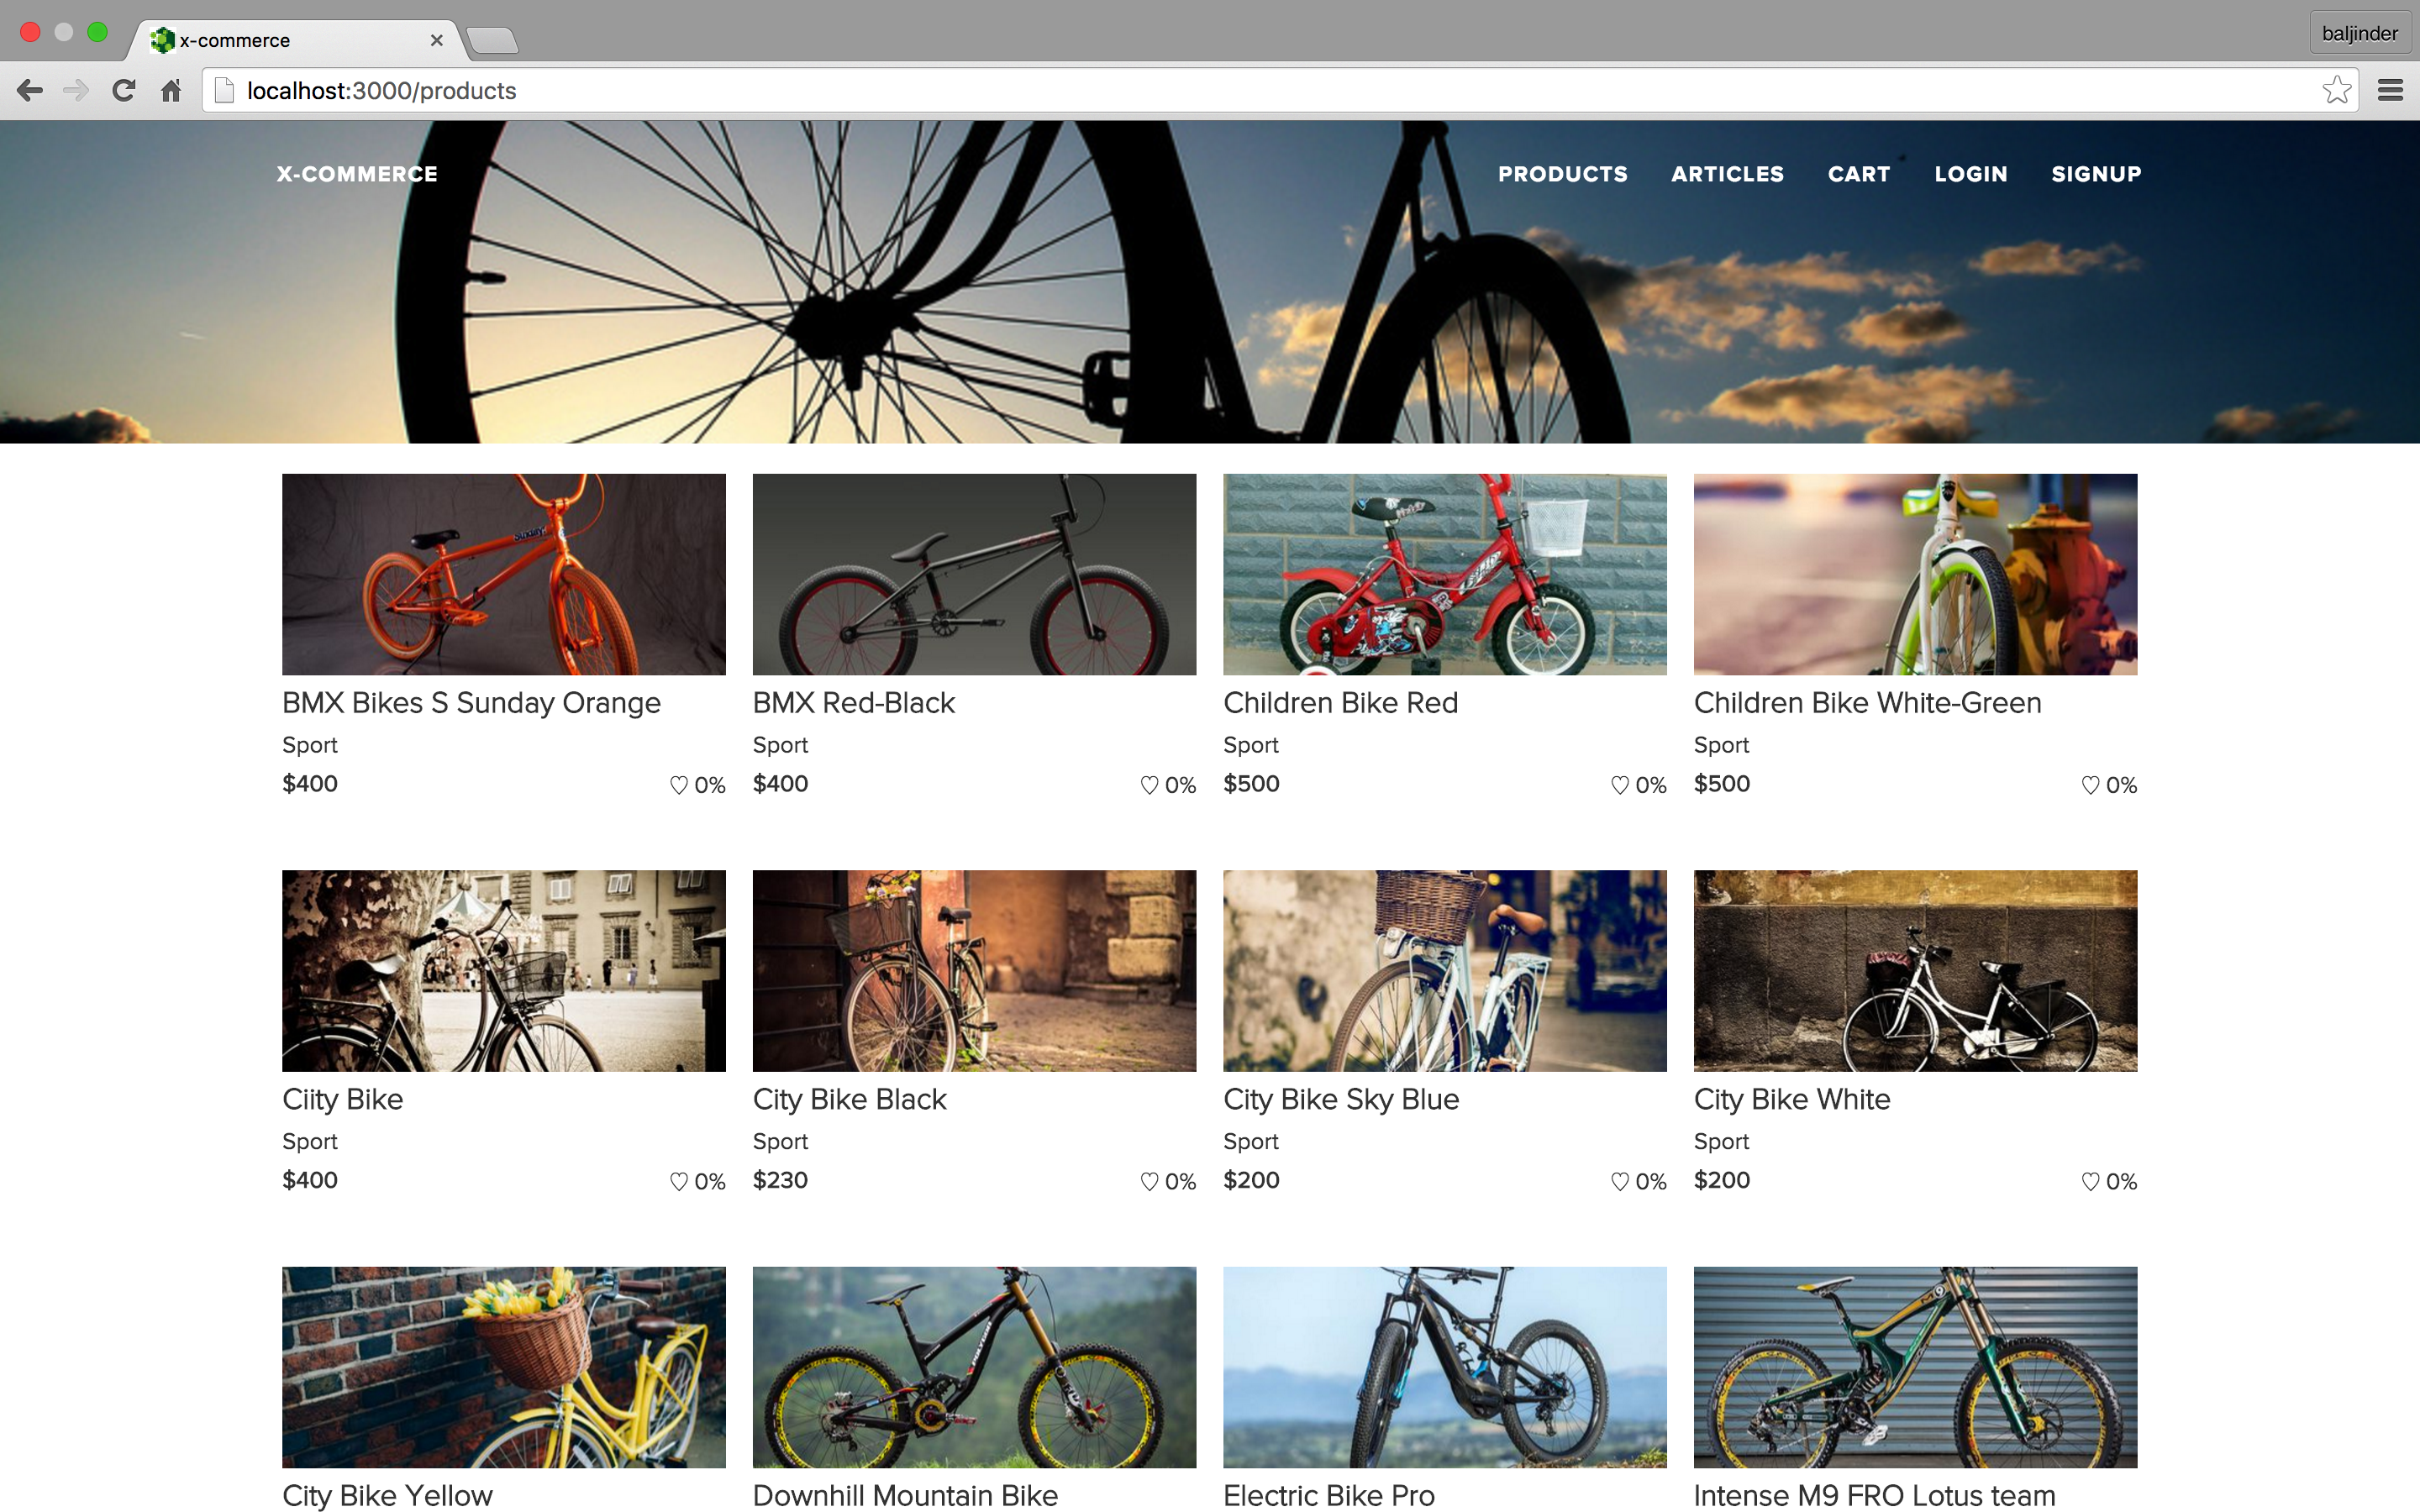
\includegraphics[width=1.0\linewidth]{images/chapter4/page-products-all-cli.png}\hfill
\caption[page products client-side]{Page products client-side}
\label{fig:page_products_client_side}
\end{figure}
Following shows the page variants of admin-side:
\begin{figure}[htb]
\centering
\includegraphics[width=1.0\linewidth]{images/chapter4/page-variants.png}\hfill
\caption[page variants admin-side]{Page variants admin-side}
\label{fig:page_variants_admin_side}
\end{figure}
Following shows the page variant of admin-side:
\begin{figure}[htb]
\centering
\includegraphics[width=1.0\linewidth]{images/chapter4/page-variant.png}\hfill
\caption[page variant admin-side]{Page variant admin-side}
\label{fig:page_variants_admin_side}
\end{figure}


